\section{Síntesis circuital}
\label{sec:sintesis}

\subsection{Función de diseño con margen}
\label{sec:margen}
La función de la plantilla $H_t(s)$ (\cref{eq:H_LP_cheb}) tiene exactamente $A_p = \qty{1}{\decibel}$ de rizado: el diseño nominal no deja margen
en la banda de paso. El circuito construido no realiza $H_t$, sino una función con $f_r$, $f_0$ y $Q$ desplazados por las tolerancias de los
componentes. Para cuantificarlo se hizo un Monte Carlo analítico sobre el circuito elegido (\cref{sec:topologia}), con distribuciones uniformes e
independientes ($R$: $\pm\qty{1}{\percent}$; $C$: $\pm\qty{5}{\percent}$ o $\pm\qty{10}{\percent}$) y \num{20000} muestras por caso, contando qué
porcentaje de los circuitos cumple la plantilla (\emph{rendimiento}).

Se compararon funciones de diseño Chebyshev~I de orden~3 con rizado $A_{p,d} \le A_p$ y borde $f_{p,d} \ge f_p$. Ambas condiciones son más
exigentes que la plantilla, de modo que el diseño nominal sigue cumpliéndola y la diferencia queda como presupuesto para las tolerancias. El precio es
una menor atenuación a \qty{4}{\kilo\hertz}, donde $H_t$ tiene casi \qty{18}{\decibel} de margen (\cref{tab:margen}).

\begin{table}[H]
  \centering\small
  \caption{Rendimiento estimado según la función de diseño (Chebyshev~I, orden~3). En negrita, la opción adoptada.}
  \label{tab:margen}
  \resizebox{\linewidth}{!}{\tabres{tab_margen}}
\end{table}

Sin margen, solo cumple alrededor del \qty{4}{\percent} de los circuitos. Se adopta la \textbf{función de diseño $H_d$: Chebyshev~I de orden~3 con
$A_{p,d} = \qty{\vApD}{\decibel}$ y $f_{p,d} = \qty{\vFpD}{\hertz}$}. Sigue siendo el filtro aprobado y eleva el rendimiento estimado al
\qty{100}{\percent} con capacitores de $\pm\qty{5}{\percent}$ y a más del \qty{98}{\percent} con $\pm\qty{10}{\percent}$, conservando
\qty{\vAcuatroD}{\decibel} de atenuación nominal a \qty{4}{\kilo\hertz} (\qty{10.7}{\decibel} de margen). Sus parámetros son
$f_r = \qty{\vFrD}{\hertz}$, $f_0 = \qty{\vFoD}{\hertz}$ y $Q = \num{\vQD}$ (\cref{fig:Ht_vs_Hd}). Toda la síntesis que sigue usa $H_d$, pero la
verificación se hace siempre contra la plantilla original.

\begin{figure}[H]
  \centering
  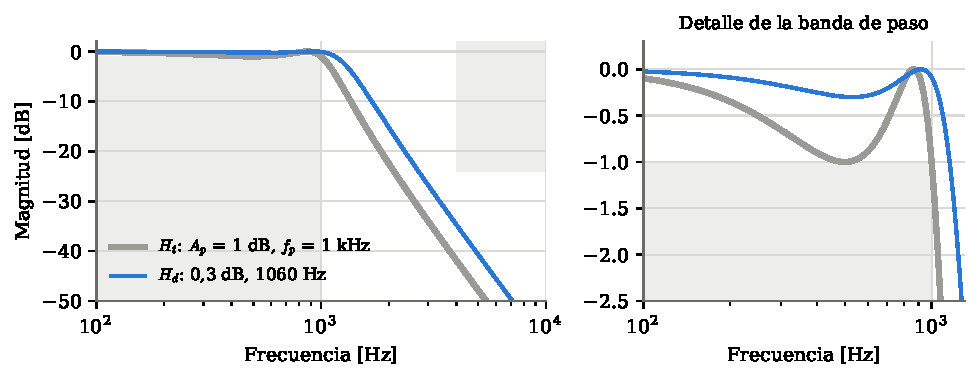
\includegraphics[width=\linewidth]{fig_Ht_vs_Hd}
  \caption{Función de la plantilla $H_t$ y función de diseño con margen $H_d$. La zona gris es la región prohibida de la plantilla.}
  \label{fig:Ht_vs_Hd}
\end{figure}

\subsection{Topología}
\label{sec:topologia}
La función de diseño se realiza en cascada (\cref{fig:esquema}), siguiendo el orden justificado en la \cref{sec:eleccion}:
\begin{itemize}
  \item \textbf{Etapa~1 (polo real):} red $R_0C_0$ seguida de un seguidor de tensión (U1). La resistencia interna del generador $R_s$
        queda en serie con $R_0$ y se incluye en el modelo.
  \item \textbf{Etapa~2 (par complejo):} Sallen--Key pasabajos~\cite[cap.~8]{daryanani1976} de ganancia unitaria ($k = 1$), con U2
        como seguidor.
\end{itemize}
Los nodos se numeran del 0 (masa) al 6 (salida); la misma numeración se usa en el netlist de LTspice.

\begin{figure}[H]
  \centering
  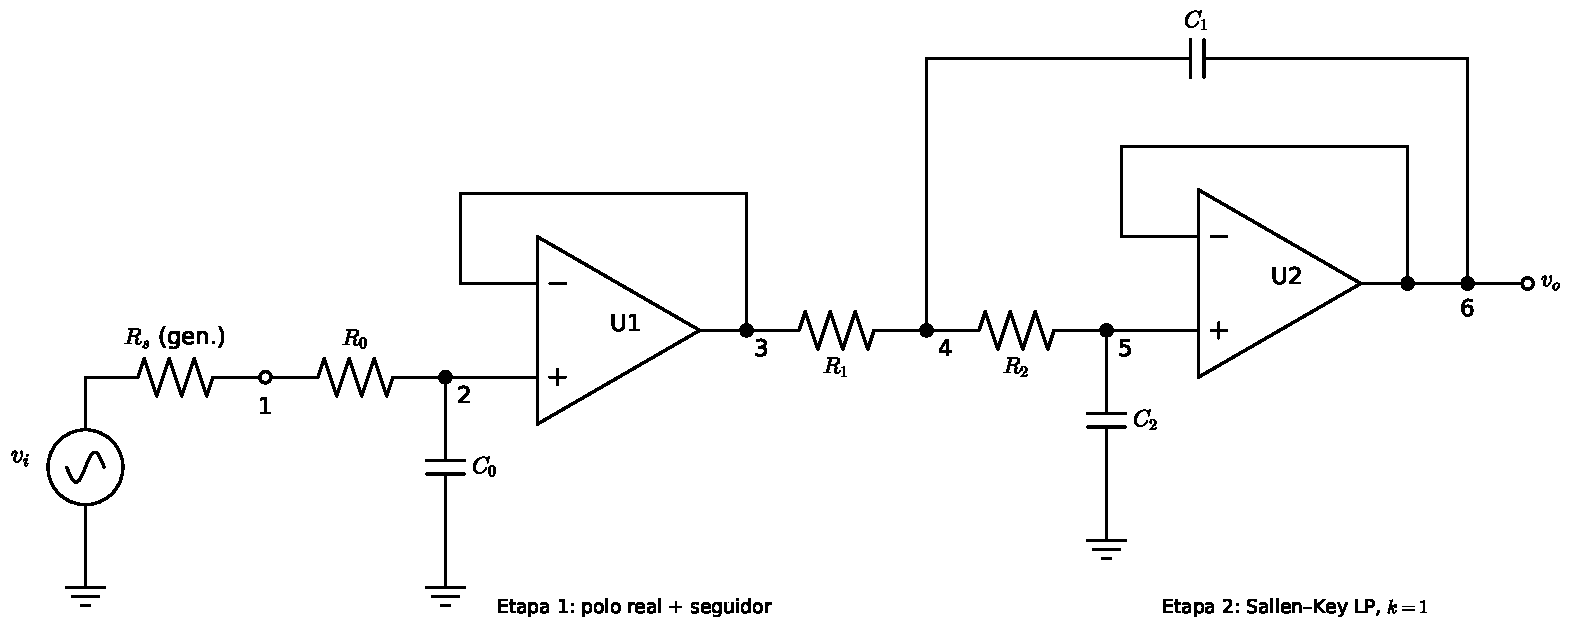
\includegraphics[width=\linewidth]{fig_esquema}
  \caption{Circuito implementado con los nodos numerados. U1 y U2 son las dos mitades de un TL072CP.}
  \label{fig:esquema}
\end{figure}

\subsection{Análisis nodal simbólico}
Con AO ideales (realimentación negativa, $v^+ = v^-$ y corrientes de entrada nulas), las ecuaciones de Kirchhoff en los nodos son
\begin{equation}
\begin{aligned}
  &\text{nodo 1:}\quad \frac{V_i-V_1}{R_s} = \frac{V_1-V_2}{R_0}, &\qquad
  &\text{nodo 2:}\quad \frac{V_1-V_2}{R_0} = sC_0V_2, &\qquad
  &\text{U1:}\quad V_3 = V_2,\\
  &\text{nodo 4:}\quad \frac{V_3-V_4}{R_1} + (V_6-V_4)\,sC_1 + \frac{V_5-V_4}{R_2} = 0, &
  &\text{nodo 5:}\quad \frac{V_4-V_5}{R_2} = sC_2V_5, &
  &\text{U2:}\quad V_6 = V_5.
\end{aligned}
\label{eq:nodales}
\end{equation}
Resolviendo el sistema con SymPy se obtiene
\begin{equation}
  H_c(s) = \frac{V_6}{V_i} =
  \underbrace{\frac{1}{sC_0(R_0+R_s)+1}}_{T_1(s)}\;
  \underbrace{\frac{1}{C_1C_2R_1R_2\,s^2 + C_2(R_1+R_2)\,s + 1}}_{T_2(s)},
  \label{eq:Hc}
\end{equation}
y, por igualación de coeficientes con las formas canónicas,
\begin{equation}
  \omega_r = \frac{1}{C_0(R_0+R_s)},\qquad
  \omega_0 = \frac{1}{\sqrt{R_1R_2C_1C_2}},\qquad
  Q = \sqrt{\frac{C_1}{C_2}}\;\frac{\sqrt{R_1R_2}}{R_1+R_2},\qquad H_c(0) = 1.
  \label{eq:param_circuito}
\end{equation}
Como $\sqrt{R_1R_2} \le (R_1+R_2)/2$, resulta $Q \le \tfrac12\sqrt{C_1/C_2}$: el Sallen--Key de ganancia unitaria exige una relación de
capacitores $n = C_1/C_2 \ge 4Q^2$, que para $H_d$ vale \num{\vCuatroQcuad}. SymPy también confirma que el caso general de ganancia
$k = 1 + r_2/r_1$ reproduce las expresiones (8.6)--(8.8) de Daryanani~\cite{daryanani1976} y que se reduce a la \cref{eq:param_circuito} con
$k = 1$. Con los valores ideales de la síntesis, $\max\lvert H_c - H_d\rvert = \num{\vErrSintesis}$: el circuito reproduce exactamente la función
de diseño.

\subsection{Aislamiento entre etapas}
Si se elimina U1, la red $R_0C_0$ queda cargada por la entrada del Sallen--Key. La diferencia entre los denominadores mónicos de ambos casos es
\begin{equation}
  D_{\text{sin U1}}(s) - D_{\text{con U1}}(s) = \frac{s\,(sC_1R_2+1)}{C_0C_1R_1R_2},
\end{equation}
que solo se anula si $R_1\to\infty$ o $C_0\to\infty$, es decir, si la segunda etapa no carga a la primera. Con los componentes elegidos, omitir el
seguidor produce un error de hasta \qty{\vErrSinBuffer}{\decibel} en la zona de \qty{1}{\kilo\hertz} (la atenuación a \qty{1}{\kilo\hertz} pasa a
ser \qty{\vAmilSinBuffer}{\decibel}, ver \cref{fig:Hc_vs_Ht}), y el filtro deja de cumplir la plantilla. Con U1, el acoplamiento queda acotado por
la impedancia de salida en lazo cerrado del AO, del orden de los miliohms a estas frecuencias, que es despreciable frente a $R_1$.

\subsection{Elección del diseño Sallen--Key}
Antes de imponer igualdades entre componentes se calcularon con SymPy las sensibilidades normalizadas
$S_x^{Q} = \frac{x}{Q}\frac{\partial Q}{\partial x}$ del Sallen--Key general respecto de sus seis elementos, y se evaluaron en los tres diseños de la
cátedra para el $Q$ de $H_d$. La \cref{tab:disenos_sk} incluye además el corrimiento de $Q$ por GBW finito, con $A(s) = \omega_t/s$.

\begin{table}[H]
  \centering
  \caption{Comparación de los diseños Sallen--Key de la cátedra~\cite[tabla~8.1]{daryanani1976} para $Q = \num{\vQD}$.}
  \label{tab:disenos_sk}
  \resizebox{\linewidth}{!}{\tabres{tab_disenos_sk}}
\end{table}

Se adopta el \textbf{diseño~1 (ganancia unitaria) en su forma generalizada}, por estos motivos:
\begin{itemize}
  \item Tiene las menores sensibilidades pasivas. Con $k = 1$ y sin imponer $R_1 = R_2$,
        \begin{equation}
          S^Q_{R_1} = -S^Q_{R_2} = \frac{R_2-R_1}{2(R_1+R_2)},\qquad S^Q_{C_1} = -S^Q_{C_2} = \frac12,\qquad
          S^{\omega_0}_{R_1,R_2,C_1,C_2} = -\frac12 ,
          \label{eq:sens_k1}
        \end{equation}
        de modo que $\lvert S^Q_{R}\rvert < \tfrac12$ para cualquier par de resistencias.
  \item No necesita la red de ganancia $r_1$, $r_2$: tiene menos componentes, $H(0) = 1$ sin ajuste de ganancia y el AO trabaja con máxima
        realimentación.
  \item El GBW finito no decide la elección: el corrimiento de $Q$ es menor que \qty{0.5}{\percent} en los tres diseños, incluso con el LM358.
\end{itemize}
La única desventaja del diseño~1 clásico ($R_1 = R_2$) es que exige $C_1/C_2 = 4Q^2$ exactamente. En la forma generalizada se eligen dos
capacitores disponibles con $n = C_1/C_2 \ge 4Q^2$ y se despejan $R_1$ y $R_2$ de la \cref{eq:param_circuito}. Ambas resistencias son las raíces
de $x^2 - x/(Q\omega_0C_2) + 1/(\omega_0^2C_1C_2) = 0$:
\begin{equation}
  R_{1,2} = \frac{1\pm\sqrt{1-4Q^2/n}}{2\,Q\,\omega_0\,C_2}.
  \label{eq:R12}
\end{equation}

\subsection{Elección de capacitores}
En el laboratorio hay capacitores de \qty{1}{\nano\farad}, \qty{4.7}{\nano\farad}, \qty{10}{\nano\farad}, \qty{47}{\nano\farad},
\qty{100}{\nano\farad} y de \qty{150}{\nano\farad} a \qty{1}{\micro\farad}, además de valores de pF (demasiado chicos para estos niveles de
impedancia) y de \qty{2.2}{\micro\farad} o más (presumiblemente electrolíticos, inadecuados para un filtro). La \cref{tab:capacitores} recorre
todos los pares disponibles con $n \ge 4Q^2$ y resistencias entre \qty{1}{\kilo\ohm} y \qty{200}{\kilo\ohm}.

\begin{table}[H]
  \centering\small
  \caption{Pares de capacitores disponibles para el Sallen--Key, ordenados por sensibilidad de $Q$ a las resistencias. La última columna es el error
  de $f_0$ si cada resistencia se redondea a un único valor E24.}
  \label{tab:capacitores}
  \tabres{tab_capacitores}
\end{table}

Se eligen $C_1 = \qty{47}{\nano\farad}$ y $C_2 = \qty{4.7}{\nano\farad}$ ($n = 10$). Es el par de menor sensibilidad,
$S^Q_{R_1} = \num{\vSQRuno}$: como $n$ queda apenas por encima de $4Q^2$, resulta $R_1 \approx R_2$, cerca del máximo de $Q$ respecto del cociente
$R_1/R_2$. Además da niveles de impedancia de unos \qty{10}{\kilo\ohm}. Para la etapa~1 se toma $C_0 = \qty{10}{\nano\farad}$, de modo que cada
valor de capacitor se usa una sola vez.

\subsection{Diseño normalizado, escaleo y resistencias}
Siguiendo el procedimiento de la cátedra~\cite{apuntes2026}, se diseña primero con $\omega_0 = \qty{1}{\radian\per\second}$ y
$C_2 = \qty{1}{\farad}$. Para $n = 10$, la \cref{eq:R12} da $R = \qty{\vRnMay}{\ohm}$ y $\qty{\vRnMen}{\ohm}$, con $C_1 = \qty{10}{\farad}$. El
escaleo de frecuencia ($k_f = \omega_0 = \qty{\vKf}{\radian\per\second}$) y de impedancia ($k_z = 1/(k_f\cdot\qty{4.7}{\nano\farad}) = \num{\vKz}$)
lleva a $C_2 = \qty{4.7}{\nano\farad}$, $C_1 = \qty{47}{\nano\farad}$, $R_1 = \qty{\vRunoId}{\kilo\ohm}$ y $R_2 = \qty{\vRdosId}{\kilo\ohm}$. El escaleo
no modifica $Q$. Para la etapa~1, $R_0 + R_s = 1/(\omega_r C_0) = \qty{\vRceroMasRs}{\kilo\ohm}$, es decir, $R_0 = \qty{\vRceroId}{\kilo\ohm}$.

Las resistencias son del \qty{1}{\percent} en valores E24. Redondear cada una a un único valor corre $f_0$ casi \qty{2}{\percent}, de modo que cada
resistencia se arma con dos valores E24 en serie (\cref{tab:resistencias}). El error residual queda en el orden de \qty{0.1}{\percent}, diez
veces menor que la tolerancia de cada resistencia.

\begin{table}[H]
  \centering\small
  \caption{Resistencias: valor ideal, redondeo a un único valor E24 y realización adoptada con dos resistencias en serie.}
  \label{tab:resistencias}
  \tabres{tab_resistencias}
\end{table}

Con $k = 1$, ambas permutaciones de $R_1$ y $R_2$ dan la misma $H_c(s)$, porque la \cref{eq:param_circuito} es simétrica, pero no los mismos niveles
internos. Con la resistencia mayor en la entrada ($R_1 = \qty{10.8}{\kilo\ohm}$), el nodo~4 alcanza como máximo $\num{\vNodoCuatroMax}\,V_i$ (frente a
$\num{\vNodoCuatroMaxAlt}\,V_i$ con la permutación) y la salida de U1 ve una impedancia mínima de \qty{\vZminUuno}{\kilo\ohm} (frente a
\qty{\vZminUunoAlt}{\kilo\ohm}).

\subsection{Verificación con valores nominales y rendimiento esperado}

\begin{table}[H]
  \centering\small
  \caption{Parámetros recalculados con los valores adoptados (AO ideal, $R_s = \qty{50}{\ohm}$) y verificación contra la plantilla.}
  \label{tab:recalculo}
  \tabres{tab_recalculo}
\end{table}

\begin{figure}[H]
  \centering
  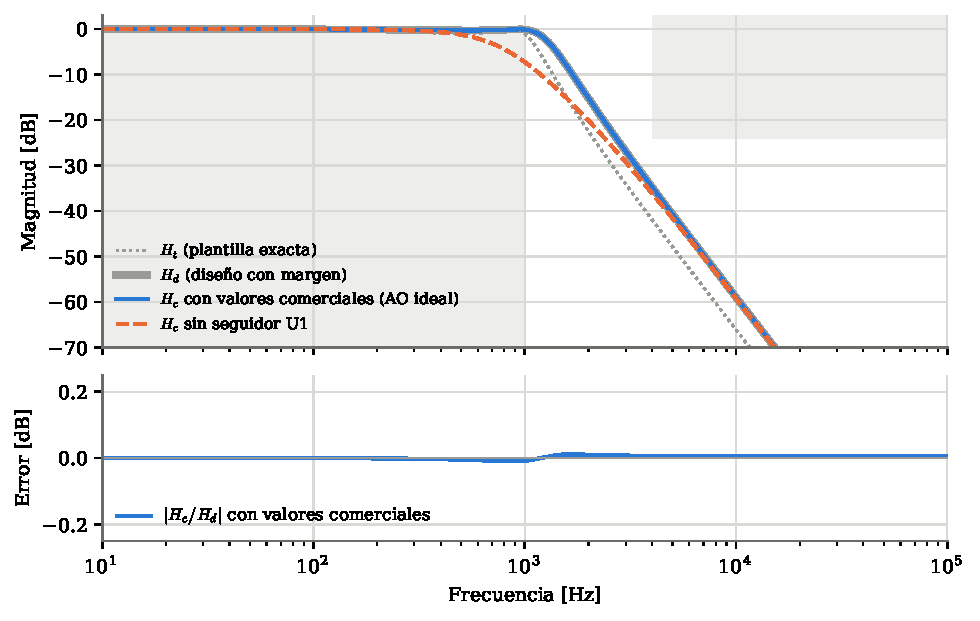
\includegraphics[width=0.92\linewidth]{fig_Hc_vs_Ht}
  \caption{Arriba: $H_t$, $H_d$, $H_c$ con los valores adoptados y $H_c$ sin el seguidor U1. Abajo: error de magnitud de $H_c$ respecto de $H_d$.}
  \label{fig:Hc_vs_Ht}
\end{figure}

Con los valores nominales, el circuito cumple la plantilla con holgura en ambas bandas: $A_{p,\max} = \qty{\vApC}{\decibel}$ frente a
\qty{1}{\decibel}, y $A(\qty{4}{\kilo\hertz}) = \qty{\vAcuatroC}{\decibel}$ frente a \qty{24}{\decibel} (\cref{tab:recalculo,fig:Hc_vs_Ht}).
Repitiendo el Monte Carlo con la realización adoptada, con cada resistencia del par en serie con su propia tolerancia, se obtiene la
\cref{tab:rendimiento} y la \cref{fig:rendimiento}. La tolerancia de los capacitores todavía no está confirmada; si fuera de
$\pm\qty{20}{\percent}$ (cerámicos de uso general), el rendimiento caería a \qty{\vRendVeinte}{\percent}. Por eso se recomiendan capacitores de film
y se verificará su código de tolerancia (J: \qty{5}{\percent}, K: \qty{10}{\percent}, M: \qty{20}{\percent}). El estudio estadístico con LTspice
corresponde al Nivel~II.

\begin{table}[H]
  \centering\small
  \caption{Rendimiento esperado de la realización adoptada ($R$: $\pm\qty{1}{\percent}$, \num{40000} muestras por caso).}
  \label{tab:rendimiento}
  \tabres{tab_rendimiento}
\end{table}

\begin{figure}[H]
  \centering
  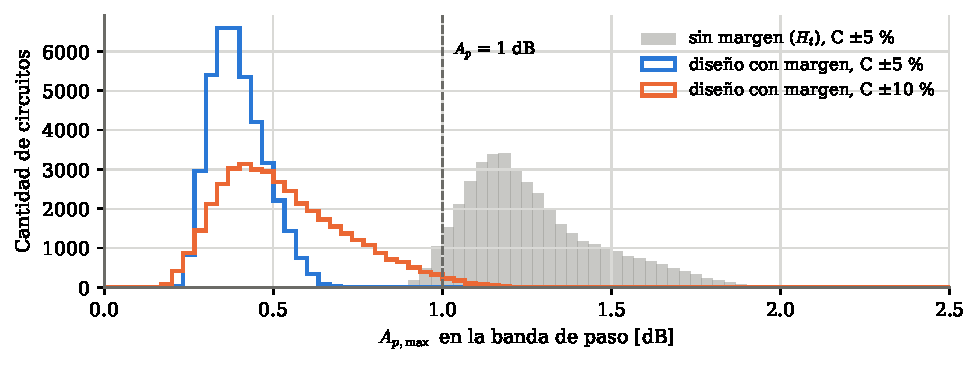
\includegraphics[width=0.9\linewidth]{fig_rendimiento}
  \caption{Distribución de la atenuación máxima en la banda de paso: síntesis sin margen ($H_t$) frente a la realización adoptada ($H_d$).}
  \label{fig:rendimiento}
\end{figure}
